\documentclass{article}
\usepackage{amsmath}
\usepackage{amsfonts}
\usepackage[inline]{enumitem}
\usepackage[a4paper,margin=1in]{geometry}
\usepackage[normalem]{ulem}
\usepackage{graphicx}
\usepackage{tasks}
\settasks{label=(\alph*), label-offset=0.4em, label-width=1.5em}

\usepackage{fancyhdr}
\fancyhf{}
\setlength{\headheight}{36pt}
\renewcommand{\headrulewidth}{0pt}
\thispagestyle{fancy}
\lhead{Calculus Exercise}
\chead{Week 4 (3.1, 3.2, 3.3, 3.4)}
\rhead{\underline{ID:\hspace{7.4em}} \\ \vspace{0.2cm} \uline{Name:\hspace{6em}}}
\cfoot{\thepage}

\begin{document}
\begin{enumerate}

    \item[3.1.86]
        Find numbers $a$ and $b$ such that the given function $g$ is differentiable at $1$.

        \begin{equation*}
            g(x) =
            \begin{cases}
                ax^3 - 3x & \text{if} \ x \leq 1\\
                bx^2 + 2 & \text{if} \ x > 1
            \end{cases}
        \end{equation*}

    \vspace{6cm}

    \item[3.1.88]

        A tangent line is drawn to the hyperbola $xy = c$ at a point $P$ as shown in the figure.
        \begin{enumerate}
            \item Show that the midpoint of the line segment cut from this tangent line by the coordinate axes is $P$.
            \item Show that the triangle formed by the tangent line and the coordinate axes always has the same area,
                no matter where $P$ is located on the hyperbola.
        \end{enumerate}

        \begin{center}
            \includegraphics[width=6cm]{./png/3.1.88.png}
        \end{center}

    \newpage


    \item[3.1.90]
        Sketch the parabolas $y = x^2$ and $y = x^2 - 2x + 2$.
        Do you think there is a line that is tangent to both curves?
        If so, find its equation. If not, why not?

    \vspace{6cm}

    \item[3.2.44]
        If $g(x)=\dfrac{x}{e^x}$, find $g^{(n)}(x)$

    \vspace{6cm}

    \item[3.2.50]
        If $f(2)=10$ and $f^{\prime}(x)=x^2f(x)$ for all $x$, find $f^{\prime\prime}(2)$.

    \newpage

    \item[3.2.58]
        Compute $Q^{\prime}(0)$, where $\displaystyle Q(x) = \frac{1+x+x^2+x e^{x}}{1 - x+ x^2 -x e^{x}}$ \\
        [12pt] \textit{Hint}: Instead of finding $Q^{\prime}(x)$ first,
        let $f(x)$ be the numerator and $g(x)$ be the denominator of $Q(x)$,
        and compute $Q^{\prime}(0)$ from $f(0)$, $f^{\prime}(0)$, $g(0)$ and $g^{\prime}(0)$.

    \vspace{6cm}

    \item[3.3.46]
        Find the limit $\displaystyle  \lim_{x \to 0 } \frac{\sin (x) }{\sin ( \pi x) }$.

    \vspace{6cm}

    \item[3.3.62]
        Find the given derivative by finding the first derivatives and observing the pattern that occurs.
        \[
            \frac{d^{35}}{dx^{35}} (x \sin (x))
        \]

    \newpage

    \item[3.3.66]
        A semicircle with diameter $PQ$ sits on an isosceles triangle $PQR$ to
        form a region shaped like a two-dimensional icecream cone, as shown in the figure.
        If $A( \theta )$ is the area of the semicircle and $B( \theta  )$ is the area of the triangle, find
        $\displaystyle  \lim_{ \theta  \to 0^{+}} \frac{A( \theta  )}{B( \theta  )}$.

        \includegraphics[width=4cm]{./png/3.3.66.png}

    \vspace{2cm}

    \item[3.4.46]
        Find the derivative of the function $\displaystyle y= \sqrt{x + \sqrt{x + \sqrt{x}}}$.

    \vspace{6cm}

    \item[3.4.48]
        Find the derivative of the function $\displaystyle y = 2^{3^{4^{x}}}$.

    \newpage

    \item[3.4.62]
        The curve $\displaystyle y = \frac{|x|}{\sqrt{2 - x^{2}}}$ is called a
        \textit{bullet-nose curve}. Find an equation of the tangent line
        to this curve at the point $(1, 1)$.

    \vspace{8cm}

    \item[3.4.69]
        A table of values for $f, g, f'$ and $g'$ is given.
        \begin{center}
            \begin{tabular}{ |c|c|c|c|c| }
                \hline
                $x$ & $f(x)$ & $g(x)$ & $f'(x)$ & $g'(x)$ \\
                \hline
                1 & 3 & 2 & 4 & 6 \\
                \hline
                2 & 1 & 8 & 5 & 7 \\
                \hline
                3 & 7 & 2 & 7 & 9 \\
                \hline
            \end{tabular}
        \end{center}

        \begin{enumerate}
            \item
                If $h(x) = f(g(x))$, find $h'(1)$.
            \item
                If $H(x) = g(f(x))$, find $H'(1)$.
        \end{enumerate}

    \newpage

    \item[3.4.99]
        Let $c$ be the $x$-intercept of the tangent line to the curve $y=b^{x}$
        ($b > 0, b \neq 1$) at the point $(a, b^{a})$. Show that the
        distance between the points $(a, 0)$ and $(c, 0)$ is the
        same for all values of $a$.

        \begin{center}
            \includegraphics[width=6cm]{./png/3.4.99.png}
        \end{center}

\end{enumerate}
\end{document}
